\documentclass[../main.tex]{subfiles}
\begin{document}

\chapter{Linear Equations}
\label{chap:chap_2}
\emph{You should be familiar with}
\begin{itemize}[noitemsep]
	\item Matrix arithmetic
	\item Linear transformations
	\item The matrix transpose and symmetric matrices
\end{itemize}

The solution of linear systems of equations is of primary importance in linear algebra. The problem of solving a linear system arises in almost all areas of engineering and science, including the structure of materials, statics and dynamics, the design and analysis of circuits, quantum physics, and computer graphics. The solution to linear systems also hides under the surface in many methods. For instance, a standard tool for data fitting is cubic splines. The fit is found by finding the solution to a system of linear equations.

This chapter introduces the basics of solving linear equations using Gaussian elimination. Since most applications deal with systems that have the same number of equations as unknowns (square systems), we will restrict our discussion to these systems. The approach we take is naive, in that it will ignore the numerical problems involved with performing Gaussian elimination on a computer. As we will see in \autoref{chap:chap:chap_8}, errors occur due to the fact that a digital computer performs arithmetic operations with a fixed number of digits. The issue of solving systems accurately is discussed in \autoref{chap:chap_11}.

\section[Introduction to Linear Equations]{INTRODUTION TO LINEAR EQUATIONS}

A \emph{linear equation} in $n$ unknowns $x_{1}, x_{2}, \ldots, x_{n}$ is an equation of the form
$$
a_{1} x_{1}+a_{2} x_{2}+\cdots+a_{n} x_{n}=b
$$
where $a_{1}, a_{2}, \ldots, a_{n}, b$ are given real numbers. For example, with $x$ and $y$ instead of $x_{1}$ and $x_{2}$, the linear equation $2 x+3 y=6$ describes the line passing through the points $(3,0)$ and $(0,2)$.

Similarly, with $x, y$, and $z$ instead of $x_{1}, x_{2}$, and $x_{3}$, the linear equation $2 x+3 y+4 z=12$ describes the plane passing through the points $(6,0,0),(0,4,0),(0,0,3)$. A system of $n$ linear equations in $n$ unknowns $x_{1}, x_{2}, \ldots, x_{n}$ is a family of equations
$$
\begin{aligned}
a_{11} x_{1}+a_{12} x_{2}+\cdots+a_{1 n} x_{n}&=b_{1} \\
a_{21} x_{1}+a_{22} x_{2}+\cdots+a_{2 n} x_{n}&=b_{2} \\
&\vdots \\
a_{n 1} x_{1}+a_{n 2} x_{2}+\cdots+a_{n n} x_{n}&=b_{n} .
\end{aligned}
$$
We wish to determine if such a system has a solution, that is to find out if there exist numbers $x_{1}, x_{2}, \ldots, x_{n}$ that satisfy each of the equations simultaneously. We say that the system is consistent if it has a solution. Otherwise, the system is called inconsistent.

Geometrically, solving a system of linear equations in two (or three) unknowns is equivalent to determining whether or not a family of lines (or planes) has a common point of intersection.


\begin{example} Solve the system
	\label{exm:exm_2_1}
	$$
	\begin{aligned}
	2 x+3 y&=6
	x-y&=2
	\end{aligned}
	$$
Multiply the second equation by 3 and add the result to the first equation.
$$5 x+0 y=12 \Longrightarrow x=12 / 5$$
Now substitute $x=12 / 5$ into the second equation to obtain $$y=x-2=\frac{12}{5}-2=\frac{2}{5}$$
The solution to the system is $x=12 / 5, y=2 / 5$.
\end{example}

In \autoref{exm:exm_2_1}, we solved the problem by dealing directly with the equations in symbolic form. This approach would be tedious and virtually unworkable for a large number of equations. We will develop a means of solving systems by using the matrix form of the equation, as discussed in \autoref{sec:sec_1_1_1}.

\begin{example} Find a polynomial of the form $y=a_{0}+a_{1} x+a_{2} x^{2}+a_{3} x^{3}$ which passes through the points $(-3,-2),(-1,2),(1,5),(2,1)$ (\autoref{fig:fig_2_1}).

When $x$ has the values $-3,-1,1,2$, then $y$ takes corresponding values $-2,2,5,1$ and we get four equations in the unknowns $a_{0}, a_{1}, a_{2}, a_{3}:$
$$
\begin{aligned}
a_{0}-3 a_{1}+9 a_{2}-27 a_{3} &=-2 \\
a_{0}-a_{1}+a_{2}-a_{3} &=2 \\
a_{0}+a_{1}+a_{2}+a_{3} &=5 \\
a_{0}+2 a_{1}+4 a_{2}+8 a_{3} &=1
\end{aligned}
$$
We will learn how to solve such a system using matrix techniques. Essentially, the process is the same as in Example 2.1. We eliminate unknowns from equations until we find one value. Using it, we are able to determine the other unknown values. The process is called Gaussian elimination. For our problem, the unique solution is
$$
\begin{aligned}
a_{0}=93 / 20, \quad a_{1}=221 / 120 \\
a_{2}=-23 / 20, \quad a_{3}=-41 / 120
\end{aligned}$$
and the required polynomial is
$$y=\frac{93}{20}+\frac{221}{120} x-\frac{23}{20} x^{2}-\frac{41}{120} x^{3}$$
\end{example}

\begin{figure}
	\centering
	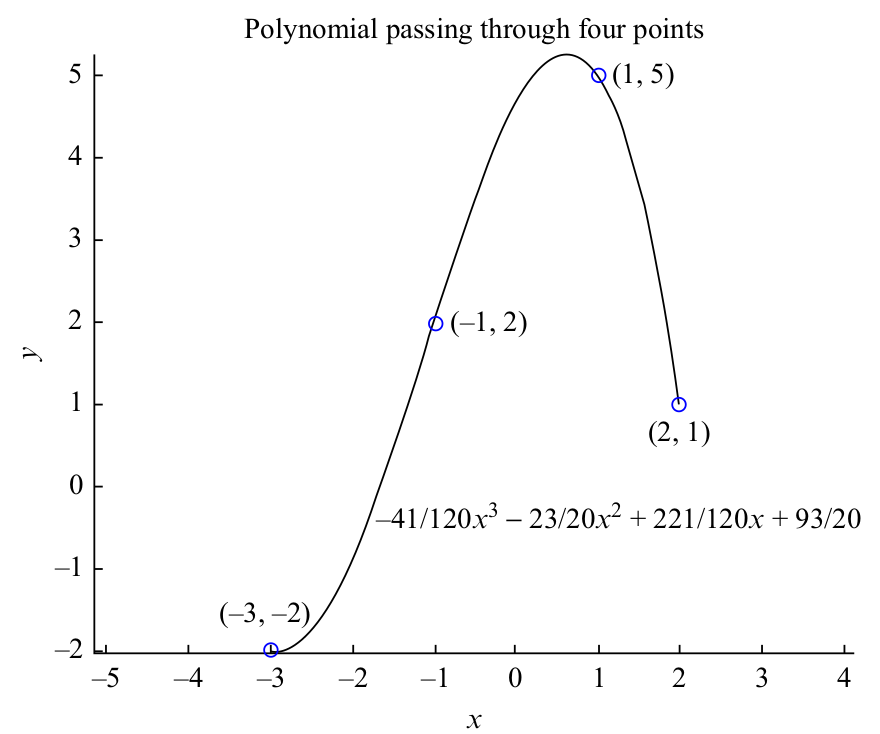
\includegraphics[width=0.7\linewidth]{fig_2_1}
	\caption{ Polynomial passing through four points.}
	\label{fig:fig_2_1}
\end{figure}

\section[Solving Square Linear Systems]{SOLVING SQUARE LINEAR SYSTEMS}
Note that the system \ref{fig:fig_2_1} can be written concisely as

\begin{equation}
	\sum_{j=1}^{n} a_{i j} x_{j}=b_{i}, \quad i=1,2, \ldots, n .
\end{equation}

We will deal with the system in matrix form. The matrix
$$
\left[\begin{array}{llll}
a_{11} & a_{12} & \ldots & a_{1 n} \\
a_{21} & a_{22} & \ldots & a_{2 n} \\
\vdots & \vdots & \ddots & \vdots \\
a_{n 1} & a_{n 2} & \ldots & a_{n n}
\end{array}\right]
$$
is called the \emph{coefficient matrix} of the system, while the matrix
$$
\left[\begin{array}{cccc|c}
a_{11} & a_{12} & \ldots & a_{1 n} & b_{1} \\
a_{21} & a_{22} & \ldots & a_{2 n} & b_{2} \\
\vdots & \vdots & \ddots & \vdots & \vdots \\
a_{n 1} & a_{n 2} & \ldots & a_{n n} & b_{n}
\end{array}\right]
$$
is called the \emph{augmented matrix} of the system. We show how to solve any square system of linear equations, using the Gaussian elimination process. Consider the following $3 \times 3$ system of equations:
$$
\begin{array}{r}
2 x_{1}+3 x_{2}-x_{3}=8 \\
-x_{1}+6 x_{2}+5 x_{3}=1 \\
9 x_{1}-5 x_{2}=4
\end{array}
$$
In matrix form, the system is written as $A x=b$, where
$$
\begin{array}{l}
A=\left[\begin{array}{ccc}
2 & 3 & -1 \\
-1 & 6 & 5 \\
9 & -5 & 0
\end{array}\right] \\
b=\left[\begin{array}{l}
8 \\
1 \\
4
\end{array}\right]
\end{array}
$$
The augmented matrix for the system is
$$
\left[\begin{array}{ccc|c}
2 & 3 & -1 & 8 \\
-1 & 6 & 5 & 1 \\
9 & -5 & 0 & 4
\end{array}\right]
$$
The matrix is really just a compact way of writing the system of equations. We now need to define some terms. The following operations are the ones used on the augmented matrix during Gaussian elimination and will not change the solution to the system. Note that performing these operations on the matrix is equivalent to performing the same operations directly on the equations.

\begin{definition}[Elementary row operations]
	\label{defn:defn_2_1}
	 Three types of \emph{elementary row operations} can be performed on matrices:
	\begin{enumerate}[label = \textbf{\arabic*.}, noitemsep]
		\item Interchanging two rows:\\
		$R_{i} \leftrightarrow R_{j}$ interchanges rows $i$ and $j .$
		\item Multiplying a row by a nonzero scalar:\\
		$R_{i} \rightarrow t R_{i}$ multiplies row $i$ by the nonzero scalar $t .$
		\item Adding a multiple of one row to another row:\\
		$R_{j} \rightarrow R_{j}+t R_{i}$ adds $t$ times row $i$ to row $j .$
	\end{enumerate}
\end{definition}

\begin{definition}[Row equivalence]
	\label{defn:defn_2_2}
	Matrix $A$ is row-equivalent to matrix $B$ if $B$ is obtained from $A$ by a sequence of elementary row operations.
\end{definition}

\begin{example} Consider the $3 \times 3$ system
$$
\begin{array}{l}
x+2 y=1 \\
2 x+y+z=3 \\
x-v+2 z=2
\end{array}
$$
In matrix form, the system is
$$
\left[\begin{array}{ccc}
1 & 2 & 0 \\
2 & 1 & 1 \\
1 & -1 & 2
\end{array}\right]\left[\begin{array}{l}
x \\
y \\
z
\end{array}\right]=\left[\begin{array}{l}
1 \\
3 \\
2
\end{array}\right]
$$
The augmented matrix is
$$
\left[\begin{array}{ccc|c}
1 & 2 & 0 & 1 \\
2 & 1 & 1 & 3 \\
1 & -1 & 2 & 2
\end{array}\right]
$$
Now begin row operations. In each case, we show the result if the operations are performed directly on the system rather than using matrix operations. You will see that performing these operations on the matrix is equivalent to performing the same operations directly on the equations. Working from left to right,

$$
\begin{aligned}
	A =
	\left[\begin{array}{ccc|c}
	1 & 2 & 0 & 1 \\
	2 & 1 & 1 & 3 \\
	1 & -1 & 2 & 2
	\end{array}\right]
	\overrightarrow{R_2 = R_2 -2 R_1 }
	\left[\begin{array}{ccc|c}
	1 & 2 & 0 & 1 \\
	0 & -3 & 1 & 1 \\
	1 & -1 & 2 & 2
	\end{array}\right]\\
	\begin{array}{cccc}
	x& +2y &&=1\\
	2x& +y& +z &= 3\\
	x & - y& +2z &= 2
	\end{array}
	\longrightarrow
	\begin{array}{cccc}
	x& +2y &&=1\\
	  & -3y& +z &= 1\\
	x & - y& +2z &= 2
	\end{array}\\
	\overrightarrow{R_2 \leftrightarrow R_3 }
	\left[\begin{array}{ccc|c}
	1 & 2 & 0 & 1 \\
	1 & -1 & 2 & 2 \\
	0 & -3 & 1 & 1
	\end{array}\right]
	\overrightarrow{R_1 = 2 R_1 }
	\left[\begin{array}{ccc|c}
	2 & 4 & 0 & 2 \\
	1 & -1 & 2 & 2 \\
	0 & -3 & 1 & 1
	\end{array}\right]\\
	\begin{array}{cccc}
		x& +2y & &=1\\
		x& -y& +2z &= 2\\
		  & -3y& +z &= 1
	\end{array}
	\longrightarrow
	\begin{array}{cccc}
		2x& +4y & &=2\\
		x& -y& +2z &= 2\\
		& -3y& +z &= 1
	\end{array}\\
\end{aligned}
$$

Thus, $A$ is row-equivalent to $B .$ Clearly, $B$ is also row-equivalent to $A$, by performing the inverse row-operations $R_{1} \rightarrow \frac{1}{2} R_{1}, R_{?} \leftrightarrow R_{3}, R_{2} \rightarrow R_{?}+2 R_{1}$ on $B$.
\end{example}

It is not difficult to prove that if $A$ and $B$ are row-equivalent augmented matrices of two systems of linear equations, then the two systems have the same solution sets-a solution of the one system is a solution of the other. For example, the systems whose augmented matrices are $A$ and $B$ in the above example are, respectively,
$$
\left\{\begin{array} { l }
{ x + 2 y = 1 } \\
{ 2 x + y + z = 3 } \\
{ x - y + 2 z = 2 }
\end{array} \quad \text { and } \quad \left\{\begin{array}{l}
2 x+4 y=2 \\
x-y+2 z=2 \\
-3 y+z=1
\end{array}\right.\right.
$$
and these systems have precisely the same solutions.


\section[Gauss Elimination]{GAUSSIAN ELIMINATION}
The augmented matrix for a system of $n$ equations and $n$ unknowns is
$$
\left[\begin{array}{cccc|c}
a_{11} & a_{12} & \ldots & a_{1 n} & b_{1} \\
a_{21} & a_{22} & \ldots & a_{2 n} & b_{2} \\
\vdots & \vdots & \ddots & \vdots & \vdots \\
a_{n 1} & a_{n 2} & \ldots & a_{n n} & b_{n}
\end{array}\right]
$$
Gaussian elimination performs row operations on the augmented matrix until the portion corresponding to the coefficient matrix is reduced to upper-triangular form.



\begin{definition}
	\label{defn:defn_2_3}An $n \times n$ matrix $A$ whose entries are of the form
$$
U_{i j}=\left\{\begin{aligned}
a_{i j}, & i \leq j \\
0, & i>j
\end{aligned}\right.
$$
is called an upper triangular matrix.
$$
U=\left[\begin{array}{cccc}
a_{11} & a_{12} & \ldots & a_{1 n} \\
0 & a_{22} & \ldots & a_{2 n} \\
\vdots & \vdots & \ddots & \vdots \\
0 & 0 & \ldots & a_{n n}
\end{array}\right]
$$
Starting with the matrix $A=\left[\begin{array}{cccc|c}a_{11} & a_{12} & \ldots & a_{1 n} & b_{1} \\ a_{21} & a_{22} & \ldots & a_{2 n} & b_{2} \\ \vdots & \vdots & \ddots & \vdots & \vdots \\ a_{n 1} & a_{n 2} & \ldots & a_{n n} & b_{n}\end{array}\right]$, row elimination produces a matrix in upper triangular form
$$
\left[\begin{array}{cccc|c}
c_{11} & c_{12} & \ldots & c_{1 n} & b_{1}^{\prime} \\
0 & c_{22} & \ldots & c_{2 n} & b_{2} \\
\vdots & \vdots & \ddots & \vdots & \vdots \\
0 & 0 & \ldots & c_{n n} & b_{n}^{\prime}
\end{array}\right]
$$
which is easy to solve.
\end{definition}

\subsection{Upper-Triangular Form}
In upper-triangular form, a simple procedure known as \emph{back substitution} determines the solution. Since the linear algebraic systems corresponding to the original and final augmented matrix have the same solution, the solution to the upper-triangular system
$$
\left[\begin{array}{cccc|c}
c_{11} & c_{12} & \ldots & c_{1 n} & b_{1}^{\prime} \\
0 & c_{22} & \ldots & c_{2 n} & b_{2}^{\prime} \\
\vdots & \vdots & \ddots & \vdots & \vdots \\
0 & \ldots & c_{n-1, n-1} & c_{n-1, n} & b_{n-1}^{\prime} \\
0 & 0 & \ldots & c_{n} & b_{n}^{\prime}
\end{array}\right]
$$
begins with
$$
x_{n}=\frac{b_{n}^{\prime}}{c_{n n}}
$$
followed by
$$
x_{n-1}=\frac{b_{n-1}^{\prime}-c_{n-1, n} x_{n}}{c_{n-1, n-1}}
$$
In general,
$$
x_{i}=\frac{b_{i}^{\prime}-\sum_{j=i+1}^{n} c_{i j} x_{j}}{c_{i i}}, \quad i=n-1, n-2, \ldots, 1 .
$$
We now formally describe the \emph{Gaussian elimination} procedure. Start with matrix $A$ and produce matrix $B$ in upper-triangular form which is row-equivalent to $A .$ If $A$ is the augmented matrix of a system of linear equations, then applying back substitution to $B$ determines the solution to the system. It is also possible that there is no solution to the system, and the row-reduction process will make this evident.

Begin at element $a_{11}$. If $a_{11}=0$, exchange rows so $a_{11} \neq 0 .$ Now make all the elements below $a_{11}$ zero by subtracting a multiple of row 1 from row $i, 2 \leq i \leq n$. The multiplier used for row $i$ is
$$\frac{a_{i 1}}{a_{1 1}}$$



The matrix is now in this form
$$
\left[\begin{array}{cccc|c}
a_{11} & a_{12} & \ldots & a_{1 n} & b_{1} \\
0 & a_{22}^{\prime} & \ldots & a_{2 n}^{\prime} & b_{2}^{\prime} \\
\vdots & \vdots & \ddots & \vdots & \vdots \\
0 & a_{n 2}^{\prime} & \ldots & a_{n n}^{\prime} & b_{n}^{\prime}
\end{array}\right]
$$
Now perform the same process of elimination by using $a_{22}^{\prime}$ and multipliers $a_{i 2}^{\prime} / a_{22}^{\prime}$, making a row exchange if necessary, so that all the elements below $a_{22}^{\prime}$ are $0 .$
$$
\left[\begin{array}{ccccc|c}
a_{11} & a_{12} & \ldots & \ldots & a_{1 n} & b_{1} \\
0 & a_{22}^{\prime} & \ldots & \ldots & a_{2 n}^{\prime} & b_{2}^{\prime} \\
\vdots & 0 & a_{33}^{\prime \prime} & \vdots & a_{3 n}^{\prime \prime} & b_{3}^{\prime} \\
0 & 0 & a_{43}^{\prime \prime} & \ddots & a_{4 n}^{\prime \prime} & b_{4}^{\prime} \\
\vdots & \vdots & \vdots & \ddots & \vdots & \vdots \\
0 & 0 & a_{n 3}^{\prime \prime} & \ldots & a_{n n}^{\prime \prime} & b_{n}^{\prime}
\end{array}\right]
$$
Repeat this process until the matrix is in upper-triangular form, and then execute back substitution to compute the solution.

\begin{example} Solve the system
$$
\begin{array}{r}
x_{1}+x_{2}-x_{3}=1 \\
2 x_{1}+x_{2}+x_{3}=0 \\
-x_{1}-2 x_{2}+3 x_{3}=2
\end{array}
$$
Row reduce the augmented matrix to upper-triangular form.
$$
\begin{array}{l}
{\left[\begin{array}{ccc|c}
	1 & 1 & -1 & 1 \\
	2 & 1 & 1 & 0 \\
	-1 & -2 & 3 & 2
	\end{array}\right] \overrightarrow{R_{2}=R_{2}-2 R_{1}}\left[\begin{array}{ccc|c}
	1 & 1 & -1 & 1 \\
	0 & -1 & 3 & -2 \\
	-1 & -2 & 3 & 2
	\end{array}\right]} \\
{\left[\begin{array}{ccc|c}
	1 & 1 & -1 & 1 \\
	0 & -1 & 3 & -2 \\
	-1 & -2 & 3 & 2
	\end{array}\right] \overrightarrow{R_{3}=R_{3}-(-1) R_{1}}\left[\begin{array}{ccc|c}
	1 & 1 & -1 & 1 \\
	0 & -1 & 3 & -2 \\
	0 & -1 & 2 & 3
	\end{array}\right]}
\end{array}
$$
$$
\left[\begin{array}{ccc|c}
1 & 1 & -1 & 1 \\
0 & -1 & 3 & -2 \\
0 & -1 & 2 & 3
\end{array}\right] \overrightarrow{R_{3}=R_{3}-(1) R_{2}}\left[\begin{array}{ccc|c}
1 & 1 & -1 & 1 \\
0 & -1 & 3 & -2 \\
0 & 0 & -1 & 5
\end{array}\right]
$$
Execute back substitution.
$$
\begin{aligned}
(-1) x_{3} &=5, \quad x_{3}=-5 \\
-x_{2}+3(-5) &=-2, \quad x_{2}=-13 \\
x_{1}+(1)(-13)-(-5) &=1, \quad x_{1}=9
\end{aligned}
$$
Final solution: $x_{1}=9, x_{2}=-13, x_{3}=-5$ When computing a solution "by hand," it is a good idea to verify that the solution is correct.
$$
\begin{array}{r}
9+(-13)-(-5)=1 \\
2(9)+(-13)+(-5)=0 \\
-(9)-2(-13)+3(-5)=2
\end{array}
$$
\end{example}


\section[Systematic Solutions of Linear Systems]{SYSTEMATIC SOLUTION OF LINEAR SYSTEMS}
Suppose a system of $n$ linear equations in $n$ unknowns $x_{1}, \ldots, x_{n}$ has augmented matrix $A$ and that $A$ is row-equivalent to a matrix $B$ in upper-triangular form. Then $A$ and $B$ have dimension $n \times(n+1)$.

\begin{enumerate}[label=Case \arabic* : ]
	\item if we perform elementary row operations on the augmented matrix of the system and get a matrix with one of its rows equal to $[000 \ldots 0 b]$, where $b \neq 0$, or a row of the form $[000 \ldots 0]$, then the system is said to be inconsistent. In this situation, there may be no solution of infinitely many solutions. In \autoref{fig:fig_2_2}, lines in the plane illustrate these two situations.

	\item There is a unique solution if Case 1 does not occur.
\end{enumerate}

\begin{example} Solve the system
$$
\begin{aligned}
x_{1}+2 x_{2} &=1 \\
2 x_{1}+x_{2}+x_{3} &=0 \\
-x_{1}+6 x_{2}+3 x_{3} &=1
\end{aligned}
$$
The augmented matrix of the system is
$$
A=\left[\begin{array}{ccc|c}
1 & 2 & 0 & 1 \\
2 & 1 & 1 & 0 \\
-1 & 6 & 3 & 1
\end{array}\right]
$$
which is row equivalent to the upper-triangular matrix
$$
B=\left[\begin{array}{ccc|c}
1 & 2 & 0 & 1 \\
0 & -3 & 1 & -2 \\
0 & 0 & \frac{17}{3} & -\frac{10}{3}
\end{array}\right]
$$
Back substitution gives the solution
$$
x_{1}=\frac{1}{17}, \quad x_{2}=\frac{8}{17}, \quad x_{3}=-\frac{10}{17}
$$
\end{example}

Solve the system
$$
\begin{array}{c}
2 x_{1}+2 x_{2}-2 x_{3}=5 \\
7 x_{1}+7 x_{2}+x_{3}=10 \\
5 x_{1}+5 x_{2}-x_{3}=5
\end{array}
$$

\begin{figure}
	\centering
	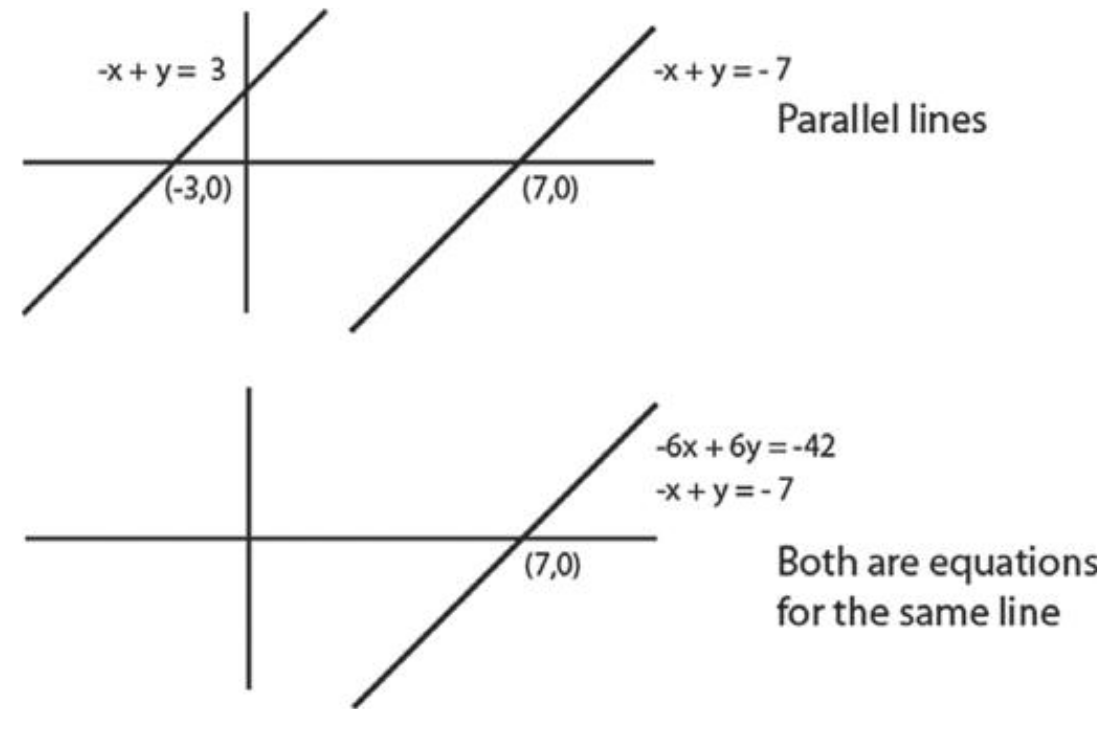
\includegraphics[width=0.7\linewidth]{fig_2_2}
	\caption{ Inconsistent equations.}
	\label{fig:fig_2_2}
\end{figure}



The augmented matrix is
$$
A=\left[\begin{array}{ccc|c}
2 & 2 & -2 & 5 \\
7 & 7 & 1 & 10 \\
5 & 5 & -1 & 5
\end{array}\right]
$$
which is row equivalent to
$$
B=\left[\begin{array}{ccc|c}
2 & 2 & -2 & 5 \\
0 & 0 & 8 & -15 / 2 \\
0 & 0 & 0 & -15 / 4
\end{array}\right]
$$
The system is inconsistent, since the last row is $[0~0~0 - 15/4]$, which implies that
$$
(0) x_{1}+(0) x_{2}+(0) x_{3}=-15 / 4
$$
The system has no solution.

\begin{example} Solve the system

\begin{align}
\label{eq:eq_2_2}
x_{1}+2 x_{2}+x_{3} &=-1,\nonumber \\
7 x_{1}+4 x_{2}+4 x_{3} &=5 \\
x_{1}+2 x_{2}+3 x_{3} &=6\nonumber
\end{align}

The augmented matrix is
$$
\left[\begin{array}{ccc|c}
1 & 2 & 1 & -1 \\
7 & 4 & 4 & 5 \\
6 & 2 & 3 & 6
\end{array}\right]
$$
Now,
$$
\begin{array}{l}
{\left[\begin{array}{ccc|c}
	1 & 2 & 1 & -1 \\
	7 & 4 & 4 & 5 \\
	6 & 2 & 3 & 6
	\end{array}\right] \overrightarrow{R_{2}=R_{2}-(7) R_{1}}\left[\begin{array}{ccc|c}
	1 & 2 & 1 & -1 \\
	0 & -10 & -3 & 12 \\
	6 & 2 & 3 & 6
	\end{array}\right]} \\
{\left[\begin{array}{ccc|c}
	1 & 2 & 1 & -1 \\
	0 & -10 & -3 & 12 \\
	6 & 2 & 3 & 6
	\end{array}\right] \overrightarrow{R_{3}=R_{3}-(6) R_{1}}\left[\begin{array}{cccc}
	1 & 2 & 1 & -1 \\
	0 & -10 & -3 & 12 \\
	0 & -10 & -3 & 12
	\end{array}\right]} \\
{\left[\begin{array}{ccc|c}
	1 & 2 & 1 & -1 \\
	0 & -10 & -3 & 12 \\
	0 & -10 & -3 & 12
	\end{array}\right] \overrightarrow{R_{3}=R_{3}-(1) R_{2}}\left[\begin{array}{ccc|c}
	1 & 2 & 1 & -1 \\
	0 & -10 & -3 & 12 \\
	0 & 0 & 0 & 0
	\end{array}\right]}
\end{array}
$$
Note that any values of $x_{1}, x_{2}$, and $x_{3}$ will satisfy
$$
\text { (0) } x_{1}+(0) x_{2}+(0) x_{3}=0
$$
Let's continue backward:
$$
-10 x_{2}-3 x_{3}=12
$$
so
$$
x_{2}=\frac{-3 x_{3}-12}{10}
$$
Substitute this relationship into the first equation of \ref{eq:eq_2_2}, and after a little algebra obtain
$$
x_{1}=\frac{-2 x_{3}+7}{5}
$$



We have determined $x_{1}$ and $x_{2}$ in terms of $x_{3}$. The complete solution is
$$
x_{1}=\frac{-2 x_{3}+7}{5}, \quad x_{2}=\frac{-3 x_{3}-12}{10},
$$
with $x_{3}$ arbitrary, so there are infinitely many solutions.
\end{example}

\begin{example} For which rational numbers $a$ and $b$ does the following system have (i) no solution, (ii) a unique solution, (iii) infinitely many solutions?
$$
\begin{aligned}
x_{1}-2 x_{2}+3 x_{3}&=4 \\
2 x_{1}-3 x_{2}+a x_{3}&=5 \\
3 x_{1}-4 x_{2}+5 x_{3}&=b
\end{aligned}
$$
The augmented matrix of the system is
$$
\begin{array}{c}
	\left[\begin{array}{ccc|c}
		1 & -2 & 3 & 4 \\
		2 & -3 & a & 5 \\
		3 & -4 & 5 & b
	\end{array}\right]\\
	\left[\begin{array}{ccc|c}
		1 & -2 & 3 & 4 \\
		2 & -3 & a & 5 \\
		3 & -4 & 5 & b
	\end{array}\right]
	\overrightarrow{\begin{subarray}{l} R_{2}=R_{2}-(2) R_{1} \\R_{3}=R_{3}-(3) R_{1} \end{subarray}}
	\left[\begin{array}{ccc|c}
		1 & -2 & 3 & 4 \\
		0 &  1 & a-6 & -3 \\
		0 &  2 & -4 & b-12
	\end{array}\right]\\
	\overrightarrow{R_{3}=R_{3}-(2) R_{2}}
	\left[\begin{array}{ccc|c}
	1 & -2 & 3 & 4 \\
	0 &  1 & a-6 & -3 \\
	0 &  0 & -2a+8 & b-6
	\end{array}\right]
	= B.
\end{array}
$$
Case 1. $a \neq 4$. Then $-2 a+8 \neq 0$ and back substitution gives a unique solution with
$$
x_{3}=\frac{b-6}{8-2 a}
$$
Case 2. $a=4$. Then
$$
B=\left[\begin{array}{ccc|c}
1 & -2 & 3 & 4 \\
0 & 1 & -2 & -3 \\
0 & 0 & 0 & b-6
\end{array}\right]
$$
If $b \neq 6$ we get no solution, whereas if $b=6$ then
$$
\begin{aligned}
x_{2}-2 x_{3} &=-3, \quad x_{2}=-3+2 x_{3} \\
x_{1}-2\left(-3+2 x_{3}\right)+3 x_{3} &=4, \quad x_{1}=-2+x_{3}
\end{aligned}
$$
The complete solution is
$x_{1}=-2+x_{3}, x_{2}=-3+2 x_{3}$, with $x_{3}$ arbitrary.
\end{example}

The MATLAB operator for solving the linear algebraic system $A x=b$ is $" \backslash "$ Use the syntax \texttt{A \textbackslash b} to obtain the solution \texttt{x}. If MATLAB detects that \texttt{A} may be singular, you will get an error message.

\begin{lstlisting}[numbers=none,frame=none]
	>> A = [1 -2 3;2 -3 4;3 -4 5];
	>> b = [4 5 7]';
	>> A\b
	Warning:	Matrix is close to singular or badly scaled.
						Results may be inaccurate. RCOND = 2.312965e-018.
	ans =
		1.0e+015 *

			-4.5036
			-9.0072
			-4.5036
	>> B = [1 5 -1;3 5 2;1 5 3]

	B =
			1	5	-1
			3	5	 2
			1	5	 3
	>> B\b

	ans =
		-0.6250
		 1.0750
		 0.7500
\end{lstlisting}



\section[Computing the Inverse]{COMPUTING THE INVERSE}
It is often useful to represent a matrix as a sequence of column vectors. If $v_{1}, v_{2}, \ldots, v_{n}$ are $n \times 1$ column vectors, the matrix $A=\left[v_{1} v_{2} \ldots v_{n}\right]$ is the $n \times n$ matrix with first column $v_{1}$, second column $v_{2}, \ldots$, and last column $v_{n} .$

Given the three column vectors $v_{1}=\left[\begin{array}{c}1 \\ -1 \\ 4\end{array}\right], v_{2}=\left[\begin{array}{l}6 \\ 0 \\ 8\end{array}\right], v_{3}=\left[\begin{array}{l}5 \\ 3 \\ 7\end{array}\right]$, then $A=\left[v_{1} v_{2} v_{3}\right]=\left[\begin{array}{ccc}1 & 6 & 5 \\ -1 & 0 & 3 \\ 4 & 8 & 7\end{array}\right]$.

This notation can also be used to represent a matrix product:
\begin{equation}
\label{eq:eq_2_3}
\begin{bmatrix}
a_{11} & \ldots & a_{1 i} & \ldots & a_{1 n} \\
a_{21} & \ldots & \vdots & \ldots & a_{2 n} \\
a_{31} & \ldots & a_{i i} & \ldots & a_{3 n} \\
\vdots & \ldots & \vdots & \ddots & \vdots \\
a_{n 1} & \ldots & a_{n i} & \ldots & a_{n n}
\end{bmatrix}
\begin{bmatrix}
b_{11} & \ldots & b_{1 i} & \ldots & b_{1 n} \\
b_{21} & \ldots & \vdots & \ldots & b_{2 n} \\
b_{31} & \ldots & b_{i i} & \ldots & b_{3 n} \\
\vdots & \ldots & \vdots & \ddots & \vdots \\
b_{n 1} & \ldots & b_{n i} & \ldots & b_{n n}
\end{bmatrix} =
\left[A\left[\begin{array}{c}
b_{11} \\
b_{21} \\
b_{31} \\
\vdots \\
b_{n 1}
\end{array}\right] \ldots A\left[\begin{array}{c}
b_{1 i} \\
\vdots \\
b_{i i} \\
\vdots \\
b_{n i}
\end{array}\right] \ldots A\left[\begin{array}{c}
b_{1 n} \\
b_{2 n} \\
b_{3 n} \\
\vdots \\
b_{n n}
\end{array}\right]\right]
\end{equation}
An example with a $2 \times 2$ matrix is easily generalized to the $n \times n$ case.
$$
A B=\left[\begin{array}{ll}
a_{11} & a_{12} \\
a_{21} & a_{22}
\end{array}\right]\left[\begin{array}{ll}
b_{11} & b_{12} \\
b_{21} & b_{22}
\end{array}\right]=\left[\begin{array}{ll}
a_{11} b_{11}+a_{12} b_{21} & a_{11} b_{12}+a_{12} b_{22} \\
a_{21} b_{11}+a_{22} b_{21} & a_{21} b_{12}+a_{22} b_{22}
\end{array}\right]=\left[A\left[\begin{array}{l}
b_{11} \\
b_{21}
\end{array}\right] A\left[\begin{array}{l}
b_{12} \\
b_{22}
\end{array}\right]\right]
$$
\autoref{eq:eq_2_3} can be used to develop a method for the computation of $A^{-1}$. Solve $n$ linear equations.
$$
A x_{i}=\left[\begin{array}{c}
0 \\
0 \\
\vdots \\
1 \\
\vdots \\
0 \\
0
\end{array}\right], \quad 1 \leq i \leq n
$$
for column vectors $x_{i} .$ In other words, find the solutions of
$$
A x_{1}=\left[\begin{array}{c}
1 \\
0 \\
0 \\
\vdots \\
0
\end{array}\right], A x_{2}=\left[\begin{array}{c}
0 \\
1 \\
0 \\
\vdots \\
0
\end{array}\right], A x_{3}=\left[\begin{array}{c}
0 \\
0 \\
1 \\
\vdots \\
0
\end{array}\right], \ldots, A x_{n}=\left[\begin{array}{c}
0 \\
0 \\
0 \\
\vdots \\
1
\end{array}\right]
$$




Now form the $n \times n$  matrix  $B$ whose first column is  $x_{1}=\begin{bmatrix}
x_{11} \\
x_{21} \\
x_{31} \\
\vdots \\
x_{n 1}
\end{bmatrix},$  whose second column is  $x_{2}=\begin{bmatrix}
x_{12} \\
x_{32} \\
x_{32} \\
\vdots \\
x_{n 2}
\end{bmatrix}$, \ldots,  and whose last column is $  x_{n}=\begin{bmatrix}x_{1 n} \\ x_{2 n} \\ x_{3 n} \\ \vdots \\ x_{n n}\end{bmatrix}$, and we have
$$
A B = A \begin{bmatrix}
x_{11} & \ldots & x_{1 i} & \ldots & x_{1 n} \\
x_{21} & \ldots & \vdots & \ldots & x_{2 n} \\
x_{31} & \ldots & x_{i i} & \ldots & x_{3 n} \\
\vdots & \ldots & \vdots & \ddots & \vdots \\
x_{n 1} & \ldots & x_{n i} & \ldots & x_{n n}
\end{bmatrix} = \begin{bmatrix}
A x_{1} & A x_{2} & \ldots & A x_{i} & A x_{n}
\end{bmatrix} =\left[\begin{array}{cccc}
\begin{bmatrix}
1 \\ 0 \\ 0 \\ \vdots \\ 0
\end{bmatrix}
\begin{bmatrix}
 0 \\ 1 \\ 0 \\ \vdots \\ 0
\end{bmatrix}
\ldots
\begin{bmatrix}
0 \\ 0 \\ 0 \\ \vdots \\ 1
\end{bmatrix}
\end{array}\right] = I.
$$

This calculation is most conveniently done by forming the augmented matrix
$$
\left[\begin{array}{ccccc|cccc}
& & & & & & & \\
a_{11} & a_{12} & \ldots & a_{1, n-1} & a_{1 n} & 1 & 0 & \ldots & 0 \\
a_{21} & a_{22} & \ldots & a_{2, n-1} & a_{2 n} & 0 & 1 & \ldots & 0 \\
\vdots & \vdots & \ddots & \vdots & \vdots & \vdots & \vdots & \ddots & \vdots \\
a_{n-1,1} & a_{n-1,2} & \ldots & a_{n-1, n-1} & a_{n-1, n} & 0 & 0 & \ldots & \vdots \\
a_{n 1} & a_{n 2} & \ldots & a_{n, n-1} & a_{n n} & 0 & 0 & \ldots & 0 \\
& & & & & 0 & 0 & \ldots & 1
\end{array}\right]
$$
and row-reducing the coefficient matrix to upper-triangular form, all the while performing the row operations on the augmented portion of the matrix. Then perform back substitution $n$ times to find $x_{1}, x_{2}, \ldots, x_{n}$

\begin{example}  Find the inverse of the matrix
$$
\begin{array}{c}
A=\left[\begin{array}{lll}
1 & 0 & 2 \\
1 & 3 & 0 \\
2 & 1 & 5
\end{array}\right] \\
{\left[\begin{array}{lll|lll}
	1 & 0 & 2 & 1 & 0 & 0 \\
	1 & 3 & 0 & 0 & 1 & 0 \\
	2 & 1 & 5 & 0 & 0 & 1
	\end{array}\right] \begin{array}{l}
	\overrightarrow{R_{2}=R_{2}-(1) R_{1}} \\
	R_{3}=R_{3}-(2) R_{1}
	\end{array}=\left[\begin{array}{lll|cll}
	1 & 0 & 2 & 1 & 0 & 0 \\
	0 & 3 & -2 & -1 & 1 & 0 \\
	0 & 1 & 1 & -2 & 0 & 1
	\end{array}\right]} \\
	\overrightarrow{R_{3}=R_{3} - \left( \frac{1}{3}\right) R_{2}}
	\left[\begin{array}{ccc|ccc}
	1 & 0 & 2 & 1 & 0 & 0 \\
	0 & 3 & -2 & -1 & 1 & 0 \\
	0 & 0 & \frac{5}{3} & -\frac{5}{3} & -\frac{1}{3} & 1
	\end{array}\right]
\end{array}
$$
Now do back substitution.
$$
\begin{aligned}
\frac{5}{3} x_{31} &=-\frac{5}{3}, \quad x_{31}=-1, \\
3 x_{21}-2 x_{31} &=-1, \quad x_{21}=\frac{2 x_{31}-1}{3}=-1, \\
x_{11}+0\left(x_{21}\right)+2 x_{31} &=1, \quad x_{11}=1-2 x_{31}=3
\end{aligned}
$$


The first column of $A^{-1}$ is $\left[\begin{array}{c}3 \\ -1 \\ -1\end{array}\right] .$ Perform back substitution two more times to obtain
$$
A^{-1}=\left[\begin{array}{ccc}
3 & \frac{2}{5} & -\frac{6}{5} \\
-1 & \frac{1}{5} & \frac{2}{5} \\
-1 & -\frac{1}{5} & \frac{3}{5}
\end{array}\right]
$$
\end{example}

Since not every matrix has an inverse, this process may fail. The matrix is singular if during back substitution you obtain a row of zeros in the coefficient matrix.

\begin{example}
$$
\begin{array}{l}
 A=\left[\begin{array}{lll}
1 & 2 & 3 \\
1 & 0 & 1 \\
3 & 4 & 7
\end{array}\right] \\
{\left[\begin{array}{lll|lll}
	1 & 2 & 3 & 1 & 0 & 0 \\
	1 & 0 & 1 & 0 & 1 & 0 \\
	3 & 4 & 7 & 0 & 0 & 1
	\end{array}\right] \begin{array}{l}
	\overrightarrow{R_{2}=R_{2}-R_{1}} \\
	R_{3}=R_{3}-3 R_{1}
	\end{array}\left[\begin{array}{ccc|ccc}
	1 & 2 & 3 & 1 & 0 & 0 \\
	0 & -2 & -2 & -1 & 1 & 0 \\
	0 & -2 & -2 & -3 & 0 & 1
	\end{array}\right]} \\
\overrightarrow{R_{3}=R_{3}-R_{2}}\left[\begin{array}{ccc|ccc}
1 & 2 & 3 & 1 & 0 & 0 \\
0 & -2 & -2 & -1 & 1 & 0 \\
0 & 0 & 0 & -2 & -1 & 1
\end{array}\right]
\end{array}
$$
There is a row of zeros. $A$ is singular.
\end{example}

\section[Homogeneous Systems]{HOMOGENEOUS SYSTEMS}
An $n \times n$ system of homogeneous linear equations
$$
\begin{aligned}
a_{11} x_{1}+a_{12} x_{2}+\cdots+a_{1 n} x_{n}=& 0 \\
a_{21} x_{1}+a_{22} x_{2}+\cdots+a_{2 n} x_{n}=& 0 \\
\vdots & \\
a_{n 1} x_{1}+a_{n 2} x_{2}+\cdots+a_{n n} x_{n}=& 0
\end{aligned}
$$
is always consistent since $x_{1}=0, \ldots, x_{n}=0$ is a solution. This solution is called the \emph{trivial solution}, and any other solution is called a \emph{nontrivial solution}. For example, consider the homogeneous system
$$
\begin{aligned}
x_{1}-x_{2}&=0,\\
x_{1} + x_{2} &= 0.
\end{aligned}
$$
Using the augmented matrix, we have
$$
\left[\begin{array}{cc|c}
1 & -1 & 0 \\
1 & 1 & 0
\end{array}\right] \overrightarrow{R_{2}=R_{2}-R_{1}}\left[\begin{array}{cc|c}
1 & -1 & 0 \\
0 & 2 & 0
\end{array}\right]
$$
so $x_{1}=x_{2}=0$, and the system has only the trivial solution. Notice that is really not necessary to attach the column of zeros.

\begin{example} Solve the homogeneous system
$$
\begin{aligned}
x_{1}+2 x_{2}+x_{3}&=0 \\
5 x_{1}+2 x_{2}+7 x_{3}&=0 \\
2 x_{1}+3 x_{3}&=0
\end{aligned}
$$




$$
\left[\begin{array}{lll}
1 & 2 & 1 \\
5 & 2 & 7 \\
2 & 0 & 3
\end{array}\right] \begin{array}{l}
\overrightarrow{R_{2}=R_{2}-5 R_{1}}\\
R_{3}=R_{3}-2 R_{1}
\end{array}\left[\begin{array}{ccc}
1 & 2 & 1 \\
0 & -8 & 2 \\
0 & -4 & 1
\end{array}\right]
\overrightarrow{R_{3}=R_{3}- {\frac{1}{2}}R_{3}} \left(\frac{1}{2}\right) R_{2}\left[\begin{array}{ccc}
1 & 2 & 1 \\
0 & -8 & 2 \\
0 & 0 & 0
\end{array}\right]
$$,
so the system has the solution $x_{1}=-\frac{3}{2} \mathrm{x}_{3}, x_{2}=x_{3} / 4$, with $x_{3}$ arbitrary. Choosing $x_{3}=1$ gives rise to the nontrivial solution
$$
x_{1}=-\frac{3}{2}, \quad x_{2}=\frac{1}{4}, \quad x_{3}=1 .
$$
\end{example}

Recall that in \autoref{chap:chap_1}, we showed that if $A$ is nonsingular, then the homogeneous system has only the trivial solution. We are now in a position to show that the reverse is also true.

\begin{theorem}
	\label{theo:theo_2_1}
	If the homogeneous system $A x=0$ has only the trivial solution, then $A$ is nonsingular; that is $A^{-1}$ exists.
\end{theorem}

\begin{proof}
	During row-reduction of the augmented matrix used to compute $A^{-1}$, there cannot be a row of zeros, or $A x=0$ would have an infinite number of solutions. As a result, back substitution will produce the inverse, and $A$ is nonsingular.
\end{proof}

\section[Application: A Truss]{APPLICATION: A TRUSS}
A truss is a structure normally containing triangular units constructed of straight members with ends connected at joints referred to as pins. Trusses are the primary structural component of many bridges. External forces and reactions to those forces are considered to act only at the pins and result in internal forces in the members, which are either tensile or compressive. Civil engineers design trusses and must determine the forces at the pins of a truss so it will remain static under a load. \autoref{fig:fig_2_3} depicts a truss under a load of 1500 units. It is allowed to move slightly horizontally at pin 1 and is static at pin $5 .$ The figure names the pins, member forces and reaction forces. There are seven member forces labeled $D$, $E, F, G, H, I$, and $J .$ A positive value for a member force means that it is a tensile force so the member force is directed away from the pins at its ends. The three reaction forces are labeled as $A, B$, and $C .$ These are due to a roller and a pinned support, and a positive value for a reaction force means that it acts in the direction shown, while a negative value means the assumed sense is wrong and should be the opposite.

The values of all these unknown (internal and reaction) forces can be found by solving a system of equations. The truss is in equilibrium, so each pin of the truss contributes two equations to the system. One equation expresses the fact that the components of the forces on that joint add to zero, and the other equation expresses the fact that the $y$ components do also. This truss contains 5 joints, labeled $1,2,3,4,5$, and thus yields 10 equations, so the resulting system of equations is $10 \times 10 .$ There is a unique solution (meaning the truss is stable) as long as the coefficient matrix is nonsingular. If the truss consists only of triangles, then this is guaranteed by the laws of statics

At pin 5, each force is either in the horizontal or vertical direction. At the remaining pins, there are both horizontal and vertical components of force, so the necessary angles must be known. If we apply the equilibrium rules, the equations for determining the truss forces are

$$
\begin{tabular}{|c|c|c|c|c|c|c|c|c|c|c|c|}
	\hline Equation & $A$ & $B$ & $C$ & $D$ & $E$ & $F$ & $G$ & $H$ & $I$ & $J$ & RHS \\
	\hline $1-x$ & 0 & 0 & 0 & $-\cos (48.4)$ & 0 & $-1$ & 0 & 0 & 0 & 0 & 0 \\
	\hline $1-y$ & $-1$ & 0 & 0 & $\sin (48.4)$ & 0 & 0 & 0 & 0 & 0 & 0 & 0 \\
	\hline $2-x$ & 0 & 0 & 0 & $-\cos (48.4)$ & $\cos (60.9)$ & 0 & 1 & 0 & 0 & 0 & 0 \\
	\hline $2-y$ & 0 & 0 & 0 & $-\sin (48.4)$ & $-\sin (60.9)$ & 0 & 0 & 0 & 0 & 0 & 0 \\
	\hline $3-x$ & 0 & 0 & 0 & 0 & $-\cos (60.9)$ & $-1$ & 0 & $\cos (45.0)$ & 0 & 1 & 0 \\
	\hline $3-y$ & 0 & 0 & 0 & 0 & $-\sin (60.9)$ & 0 & 0 & $-\sin (45.0)$ & 0 & 0 & 1500 \\
	\hline $4-x$ & 0 & 0 & 0 & 0 & 0 & 0 & $-1$ & $-\cos (45.0)$ & 0 & 0 & 0 \\
	\hline $4-y$ & 0 & 0 & 0 & 0 & 0 & 0 & 0 & $-\sin (45.0)$ & $-1$ & 0 & 0 \\
	\hline $5-x$ & 0 & $-1$ & 0 & 0 & 0 & 0 & 0 & 0 & 0 & $-1$ & 0 \\
	\hline $5-y$ & 0 & 0 & $-1$ & 0 & 0 & 0 & 0 & 0 & 1 & 0 & 0 \\
	\hline
\end{tabular}
$$


\begin{figure}
	\centering
	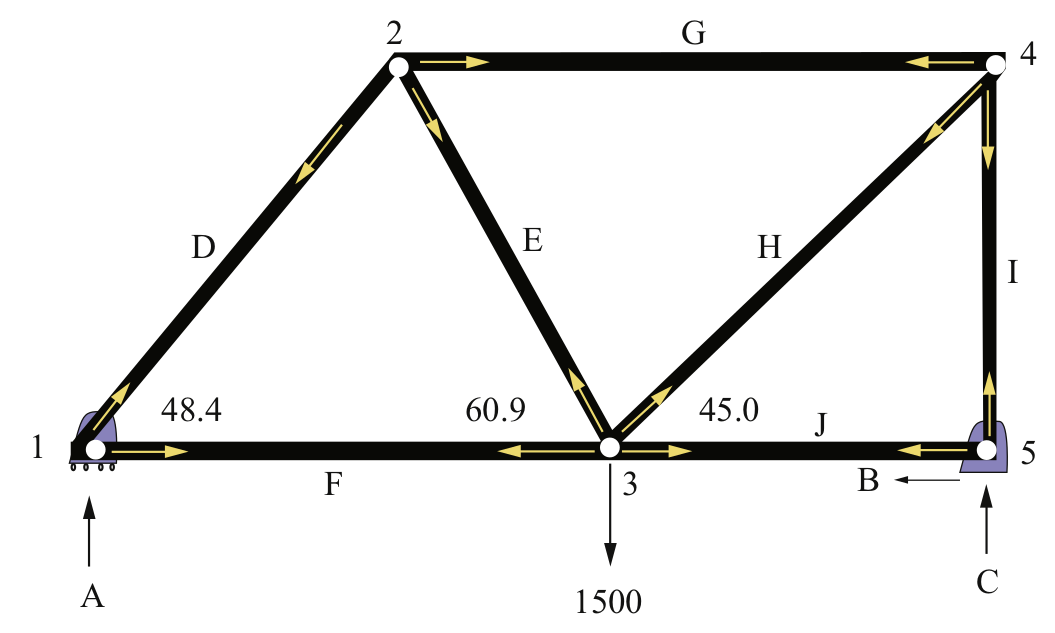
\includegraphics[width=0.7\linewidth]{fig_2_3}
	\caption{ Truss.}
	\label{fig:fig_2_3}
\end{figure}
These equations correspond to the matrix formulation
$$\left[\begin{array}{cccccccccc}0 & 0 & 0 & -0.6639 & 0 & -1 & 0 & 0 & 0 & 0 \\ -1 & 0 & 0 & 0.7478 & 0 & 0 & 0 & 0 & 0 & 0 \\ 0 & 0 & 0 & -0.6639 & 0.4863 & 0 & 1 & 0 & 0 & 0 \\ 0 & 0 & 0 & -0.7478 & -0.8738 & 0 & 0 & 0 & 0 & 0 \\ 0 & 0 & 0 & 0 & -0.4863 & -1 & 0 & 0.7071 & 0 & 1 \\ 0 & 0 & 0 & 0 & -0.8738 & 0 & 0 & -0.7071 & 0 & 0 \\ 0 & 0 & 0 & 0 & 0 & 0 & -1 & -0.7071 & 0 & 0 \\ 0 & 0 & 0 & 0 & 0 & 0 & 0 & -0.7071 & -1 & 0 \\ 0 & -1 & 0 & 0 & 0 & 0 & 0 & 0 & 0 & -1 \\ 0 & 0 & -1 & 0 & 0 & 0 & 0 & 0 & 1 & 0\end{array}\right]\left[\begin{array}{l}A \\ B \\ C \\ D \\ E \\ F \\ G \\ H \\ I \\ J\end{array}\right]=\left[\begin{array}{l}0 \\ 0 \\ 0 \\ 0 \\ 0 \\ 1500 \\ 0 \\ 0 \\ 0 \\ 0\end{array}\right] .$$
Note that the coefficient matrix contains mostly zeros, so it is a sparse matrix.

The software distribution contains two files, \texttt{TRUSS.mat} and \texttt{TRUSS.txt}. \texttt{TRUSS.mat} is the truss coefficient matrix in internal MATLAB format, and \texttt{TRUSS.txt} is a text file representation of the matrix. After reading in the matrix using either file and applying the MATLAB " $\backslash$ "operator, the solution is

$$
\left[\begin{array}{c}
A \\ B \\ C\\ D\\ E\\ F\\ G\\ H\\ I\\
\end{array}\right] =
\left[ \begin{array}{c}
613.66\\ 0.0\\ 886.34\\ 820.62\\ -702.29\\ -544.81\\
886.34\\ -1253.5 \\886.34 \\0.0
\end{array}\right]
$$

\begin{lstlisting}[numbers=none,frame=none]
	>> load Truss
	>> format shortg % output looks better
	>> rhs = zeros(10,1);
	>> rhs(6) = 1500;
	>> Truss\rhs
	ans =
				 613.66
							0
				 886.34
				 820.62
				-702.29
				-544.81
				 886.34
				-1253.5
				 886.34
							0
\end{lstlisting}



\section[Application: Eletrical Circuit]{APPLICATION: ELECTRICAL CIRCUIT}
\autoref{fig:fig_2_4} is a diagram of a DC electric circuit containing batteries and resistors. The voltage across a resistor in a circuit is determined using Ohm’s Law, $V = RI$, where $R$ is the resistance and $I$ is the current. We would like to determine the currents $i_{i}, i_{2}, i_{3}$. The currents can be determined by using \emph{Kirchhoff ’s rules}, which state that

\begin{enumerate}[noitemsep, label=textbf{\arabic*.}]
	\item At any junction point in a circuit where the current can divide, the sum of the currents into the junction must equal the sum of the currents out of the junction.
	\item  When any closed loop in the circuit is traversed, the sum of the changes in voltage must equal zero.
\end{enumerate}

Rule 1 is called the \emph{Kirchhoff ’s Current Law}, and is a consequence of conservation of charge. Rule 2 is termed the \emph{Kirchhoff ’s Voltage Law}, and is a consequence of the conservation of energy. In the circuit of \autoref{fig:fig_2_4}, there are two
junction points $A$ and $B$ and two loops. What we must do is apply Kirchhoff’s rules to obtain a system of equations that will allow us to find the current values. Before we can begin, the direction of the current in each branch must be assigned. Once this is done, appropriate signs must be given to each resistor and voltage. Label the side of a resistor on which the
current enters as positive ($+$) and the side on which the current exits as negative ($-$). It can be difficult to determine in which direction the current actually flows. If the direction is not correct, the current will be negative in that branch. Note the choices made for the circuit of \autoref{fig:fig_2_4} It is now time to apply Kirchhoff’s rules as follows:
\begin{enumerate}[noitemsep, label=\textbf{\arabic*.}]
	\item Apply the first rule to all but one junction point. Each time you use the first rule, a current not already used must be included; otherwise, you will have redundant equations.
	\item Apply the second rule to enough loops so the currents in the loop equations and those in the junction equations equal the number of unknown currents.
\end{enumerate}
We will now determine the equations for the circuit in \autoref{fig:fig_2_4}

Apply rule 1 at junction A: i1 + i3 = i2.

In the two applications of the loop rule, note that the signs in each equation are determined by whether the current moves from $+$ to $-$ or $-$ to $+$.

Apply rule 2 to loop 1: $-V_{1} + R_{1}i_{1} + R_{2}i_{2} + V_{2} + R_{4}i_{1} = 0, \text{and} (R_{1} + R_{4})i_{1} + R_{2}i_{2} = V_{1} - V_{2}$

Apply rule 2 to loop 2:  $R_{2}i_{2} + V_{2} -V_{3} + R_{3}i_{3} = 0, \text{and} (R_{2} i_{2} + R_{3})i_{3}  = V_{3} - V_{2}$

We now have three equations and three unknowns:
\begin{align}
	\label{eq:eq_2_4}
	i_{1} - i_{2} + i_{3} &= 0, \nonumber \\
	(R_{1} + R_{4}) i_{1} + R_{2}i_{2} &= V_{1} - V_{2},\\
	R_{2}i_{2} + R_{3}i_{3} &= V_{3} - V_{2}.\nonumber
\end{align}

\begin{figure}
	\centering
	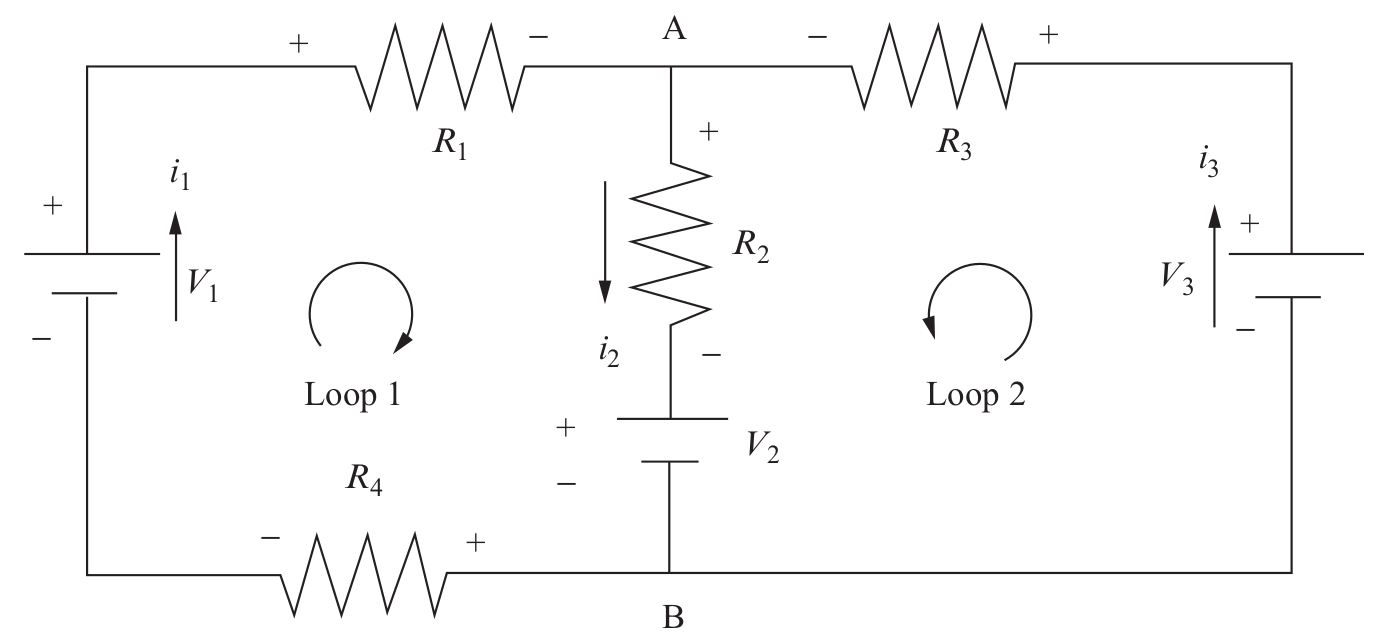
\includegraphics[width=0.7\linewidth]{fig_2_4}
	\caption{Electrical circuit.}
	\label{fig:fig_2_4}
\end{figure}




Choose the following values for the batteries and the resistors:

\begin{tabular}{|l|c|c|c|c|c|c|c|}
	\hline Components & $V_{1}$ & $V_{2}$ & $V_{3}$ & $R_{1}$ & $R_{2}$ & $R_{3}$ & $R_{4}$ \\
	\hline & $2 \mathrm{~V}$ & $3 \mathrm{~V}$ & $5 \mathrm{~V}$ & $1 \Omega$ & $2 \Omega$ & $5 \Omega$ & $3 \Omega$ \\
	\hline
\end{tabular}

\autoref{eq:eq_2_4} then becomes
$$
\begin{aligned}
i_{1}-i_{2}+i_{3} &=0 \\
4 i_{1}+2 i_{2} &=-1 \\
2 i_{2}+5 i_{3} &=2
\end{aligned}
$$
In matrix form, the system is $\left[\begin{array}{ccc}1 & -1 & 1 \\ 4 & 2 & 0 \\ 0 & 2 & 5\end{array}\right]\left[\begin{array}{l}i_{1} \\ i_{2} \\ i_{3}\end{array}\right]=\left[\begin{array}{c}0 \\ -1 \\ 2\end{array}\right]$, and the currents are
$$
i_{1}=-0.2895, \quad i_{2}=0.0789, \quad i_{3}=0.3684
$$
Note that $i_{1}$ flows in the direction opposite to what is shown in \autoref{fig:fig_2_4}.

\section[Chapter Summary]{CHAPTER SUMMARY}

\subsection*{Introduction to Linear Equations}
A system of $n$ linear equations in $n$ unknowns $x_{1}, x_{2}, \ldots, x_{n}$ is a family of equations
$$
\begin{aligned}
a_{11} x_{1}+a_{12} x_{2}+\cdots+a_{1 n} x_{n}&=b_{1} \\
a_{21} x_{1}+a_{22} x_{2}+\cdots+a_{2 n} x_{n}&=b_{2} \\
&\vdots \\
a_{n 1} x_{1}+a_{n 2} x_{2}+\cdots+a_{n n} x_{n}&=b_{n}
\end{aligned}
$$
Determine if there exist numbers $x_{1}, x_{2}, \ldots, x_{n}$ which satisfy each of the equations simultaneously. To determine a solution using Gaussian elimination, multiply an equation by a constant and subtract from another equation in order to eliminate an unknown. Do this in an organized fashion until obtaining an equation containing only one unknown. Compute it and then execute a process of substitution to determine the remaining unknowns. It is tedious to do this by writing down equations, and we want an approach that we can implement on a computer. The solution is to write the system in matrix form $A x=b$, where $A$ is the matrix of coefficients and to perform matrix operations, something a computer can do very well.

\subsection*{Solving Square Linear Equations}
Given a matrix $A$, there are three fundamental operations we can perform:
\begin{itemize}[noitemsep]
	\item  Multiply a row by constant.
	\item Exchange two rows.
	\item Multiply a row by a constant and subtract it from another row.
\end{itemize}

These are termed elementary row operations, and a matrix produced by one or more of these operations is said to be row equivalent to the original matrix. The approach we take to solving linear systems is to attach the right-hand sides as an additional colnmn to form an $n \times(n+1)$ matrix. This is called the angmented matrix. Performing elementary row operations with this matrix is equivalent to performing the same operations directly on the equations. If we transform the augmented matrix



$$
\left[\begin{array}{ccccc|c}
a_{11} & a_{22} & \ldots & a_{1, n-1} & a_{1 n} & b_{1} \\
a_{21} & a_{22} & \ldots & a_{2, n-1} & a_{2 n} & b_{2} \\
\vdots & \vdots & \ddots & \vdots & \vdots & \vdots \\
\vdots & \vdots & \vdots & \ddots & \vdots & b_{n-1} \\
a_{n 1} & a_{n 2} & \ldots & a_{n, n-1} & a_{n n} & b_{n}
\end{array}\right]
$$
to a matrix
$$
\left[\begin{array}{ccccc|c}
\bar{a}_{11} & \bar{a}_{12} & \ldots & \bar{a}_{1, n-1} & \bar{a}_{1 n} & \bar{b}_{1} \\
\bar{a}_{21} & \bar{a}_{22} & \ldots & \bar{a}_{2, n-1} & \bar{a}_{2 n} & \bar{b}_{2} \\
\vdots & \vdots & \ddots & \vdots & \vdots & \vdots \\
\vdots & \vdots & \vdots & \ddots & \vdots & \vdots \\
\bar{a}_{n 1} & \bar{a}_{n 2} & \ldots & \bar{a}_{n, n-1} & \bar{a}_{n n} & \bar{b}_{n}
\end{array}\right]
$$
the two systems have the same solutions.

\subsection*{Gaussian Elimination}
To execute Gaussian elimination, create the augmented matrix and perform row operations that reduce the coefficient matrix to upper-triangular form. The solution to the upper-triangular system is the same as the solution to the original linear system Solve the upper-triangular system by back substitution, as long as the element at position $(n, n)$ is not zero. The unknown $x_{n}$ is immediately available using the last row of the augmented matrix. Using $x_{n}$ in the equation represented by row $n-1$. we find $x_{n-1}$, and so forth, until determining $x_{1}$. If position $(n, n)$ is zero, then the entire last row of the coefficient matrix is zero, and there is either no solution or infinitely many solutions.

\subsection*{Systematic Solution of Linear Equations}
One method of solving a linear system $A x=b$ is reduction to upper triangular form. If $a_{11}=0$, exchange rows so it is nonzero. Multiply row 1 by $a_{21} / a_{11}$ and subtract from row $2 .$ That zeros-out the element in row 2, column $1 .$ Now multiply row 1 by $a_{31} / a_{11}$ and subtract from row 3 , zeroing out the element in row 3 , column 1. Continue until zeroing-out $a_{1 n}$. The first column now has the form
$$
\left[\begin{array}{c}
a_{11} \\
0 \\
\vdots \\
0
\end{array}\right]
$$
Move down one row and over one column to position $(2,2) .$ Make sure the element there, $\bar{a}_{22}$, is nonzero; if not, swap rows. Using $\bar{a}_{22}$. zero-out the elements at positions $(3.2) \cdot(4,2) \ldots(n .2)$. Move to row 3. column 3 and repeat the process. Aftcr proccssing $n-1$ columns the augmcntcd matrix is in upper-triangular form
$$
\left[\begin{array}{cccc|c}
c_{11} & c_{12} & \ldots & c_{1 n} & b_{1}^{\prime} \\
0 & c_{22} & \ldots & c_{2 n} & b_{2}^{\prime} \\
\vdots & \vdots & \ddots & \vdots & \vdots \\
0 & 0 & \ldots & c_{n n} & b_{n}^{\prime}
\end{array}\right]
$$
Perform back substitution to compute the unique solution, if it exists.

If the last row of the reduced coefficient matrix is all zeros, and the corresponding element of the augmented column is nonzero, the system has no solution; otherwise, there are infinitely many solutions.

\subsection*{Computing the Inverse}
To compute the inverse, attach the $n$ columns of the identity matrix to form an augmented matrix. By performing elementar row operations on the entire augmented matrix, reduce the coefficient matrix portion to upper-triangular form. Perform back substitution once for every attached column that was produced from the identity matrix. The solution obtained from the original right-hand side
$
\left[\begin{array}{c}
1\\ 0 \\ \vdots \\ 0
\end{array}\right]
$
is the first column of the inverse. Continue in the same fashion to obtain columns $2 - n$ of the inverse.

\subsection*{Homogeneous Systems}
To solve a system of the form $Ax = 0$, there is no reason to form the augmented matrix, since all components will remain zero during row elimination. After reduction to upper-triangular form, if the element in position $(n, n)$ is nonzero, the system has the unique solution $x = 0$; otherwise, there is an infinite number of solutions, and the matrix $A$ is singular.

\subsection*{Applications}
A truss presents a problem in statics. Forces must balance so the truss remains intact under a given load or loads. At the pins, the force-in must equal the force-out. If there are $k$ pins, a system with $2k$ equations and $2k$ unknowns results, where
the right-hand side is formed from the loads. A solution of the system gives the forces at the pins.

If an electrical circuit has one or more batteries and consists entirely of resistors, the currents in the circuit are found by solving a linear system determined by using the relationship $V = RI$ for every resistor and applying Kirchhoff’s rules.

\section[Problems]{ PROBLEMS}
\begin{enumerate}[label=\textbf{2.\arabic*}]

\item Find the unique solution to each system of linear equations.

	\begin{enumerate}[label=\textbf{\alph*.}]
	\item $2x + y = 3\\
				x - y = 1$
	\item $x_1 + 2x_2 + x_3 = 1\\
				x_2 - x_3 = 0\\
				x_1 + 2x_2 + 2x_3 = 1$
	\end{enumerate}

\item Solve the following systems of linear equations by reducing the augmented matrix to upper-triangular form:

		\begin{enumerate}[label=\textbf{\alph*.}]
		\item $a. x_1 + x_2 + x_3 = 2\\
					2x_1 + 3x_2 - x_3 = 8\\
					x_1 - x_2 - x_3 = -8$
		\item $2x_2+3x_3 - 4x_4 = 1\\
					2x_3+3x_4 = 4\\
					2x_1 + 2x_2 - 5x_3 + 2x_4 = 4\\
					2x_1 - 6x_3+9x_4= 7$
		\end{enumerate}

\item Show that the following system is consistent if $c = 2a - 3b$ and solve the system in this case.
$$
\begin{aligned}
2x - y+3z &= a\\
3x + y - 5z &= b\\
-5x - 5y+21z &= c
\end{aligned}
$$

\item Solve the homogeneous system
$$\begin{aligned}
-3x_1 + x_2 + x_3 + x_4 &= 0\\
x_1 - 3x_2 + x_3 + x_4 &= 0\\
x_1 + x_2 - 3x_3 + x_4 &= 0\\
x_1 + x_2 + x_3 - 3x_4 &= 0.
\end{aligned}$$

\item For which rational numbers $\lambda$ does the homogeneous system
$$\begin{aligned}
	x + (\lambda - 3)y &= 0\\
	(\lambda - 3)x + y &= 0
\end{aligned}$$
have a nontrivial solution?


\item Let $A=\left[\begin{array}{ll}a & b \\ c & d\end{array}\right]$. Show that $A$ is row-equivalent to $\left[\begin{array}{ll}1 & 0 \\ 0 & 1\end{array}\right]$ if $a d-b c \neq 0$, but is row-equivalent to a matrix whose second row is zero, if $a d-b c=0$.

\item For which rational numbers $a$ does the following system have (i) no solutions, (ii) exactly one solution, (iii) infinitely many solutions?
$$
\begin{aligned}
&x_{1}+2 x_{2}-3 x_{3}=4 \\
&3 x_{1}-x_{2}+5 x_{3}=2 \\
&4 x_{1}+x_{2}+\left(a^{2}-14\right) x_{3}=a+2
\end{aligned}
$$

\item Find the rational number $k$ for which the matrix $A=\left[\begin{array}{ccc}1 & 2 & k \\ 3 & -1 & 1 \\ 5 & 3 & -5\end{array}\right]$ is singular


\item Show that the matrix $A=\left[\begin{array}{ccc}1 & a & b \\ -a & 1 & c \\ -b & -c & 1\end{array}\right]$ is nonsingular by demonstrating that $A$ is row-equivalent to $\mathrm{L}$.


\item Find the inverse, if it exists, for each matrix.

	\begin{enumerate}[label=\textbf{\alph*.}]
	\item  $\left[\begin{array}{ll}1 & 3 \\ 0 & 2\end{array}\right]$
	\item $\left[\begin{array}{ll}1 & 3 \\ 2 & 6\end{array}\right]$
	\item $\left[\begin{array}{ccc}1 & -1 & 2 \\ 0 & 1 & 3 \\ 0 & 4 & 2\end{array}\right]$
	\item $\left[\begin{array}{cccc}1 & 2 & 0 & 0 \\ 1 & 3 & -1 & 0 \\ 0 & -1 & 1 & 3 \\ 0 & 0 & 2 & 3\end{array}\right]$
	\item $\left[\begin{array}{cccc}1 & 2 & 0 & 0 \\ 1 & 1 & -1 & 0 \\ 0 & -1 & 1 & 3 \\ 0 & 0 & 2 & 3\end{array}\right]$
	(e) and (d) differ only in row 2, column 2. Note the huge difference!
	\item What type of matrices are those in (d) and (e)?
\end{enumerate}

\end{enumerate}

\subsection{ MATLAB Problems}

\begin{enumerate}[label=\textbf{2.\arabic*}]
	\addtocounter{enumi}{10}
\item Use MATLAB to solve the linear algebraic system
$$
\left[\begin{array}{cccc}
1 & 3 & 8 & 0 \\
-1 & -12 & 3 & 1 \\
15 & 3 & 5 & 6 \\
55 & 2 & 35 & 5
\end{array}\right]\left[\begin{array}{l}
x_{1} \\
x_{2} \\
x_{3} \\
x_{4}
\end{array}\right]=\left[\begin{array}{l}
1 \\
0 \\
2 \\
3
\end{array}\right]
$$

\item Solve the system $H x=[11 \ldots 1]^{\mathrm{T}}$, where $H$ is the $20 \times 20$ Hilbert matrix discussed in \textcolor{blue}{Problem \ref{pro:pro_1_28}} of \autoref{chap:chap_1} . Now solve the system $H x=\left[\begin{array}{llll}0.99 & 0.99 & \ldots & 0.99\end{array}\right]^{\mathrm{T}}$. Discuss the results.

In algebra, the polynomial $x^{2}-5 x+6$ can be factored as $(x-3)(x-2)$. Under the right conditions, a matrix can also be factored. Exercises $2.13$ and $2.14$ are designed to introduce you to \emph{matrix factorization}, a topic of great importance in numerical linear algebra.



\item  A \emph{bidiagonal matrix} is a matrix with nonzero entries along the main diagonal and either the diagonal above or the diagonal below. The matrix $B 1$ is an \emph{upper bidiagonal matrix} and $B 2$ is a \emph{lower bidiagonal matrix}.
$$
B 1=\left[\begin{array}{llll}
5 & 1 & 0 & 0 \\
0 & 5 & 2 & 0 \\
0 & 0 & 5 & 3 \\
0 & 0 & 0 & 5
\end{array}\right], \quad B 2=\left[\begin{array}{cccc}
5 & 0 & 0 & 0 \\
-1 & 5 & 0 & 0 \\
0 & -2 & 5 & 0 \\
0 & 0 & -3 & 5
\end{array}\right].
$$
A \emph{tridiagonal matrix} has only nonzero entries along the main diagonal and the diagonals above and below. $T$ is a tridiagonal matrix.
$$
T=\left[\begin{array}{ccccc}
5 & -1 & 0 & 0 & 0 \\
1 & 5 & -1 & 0 & 0 \\
0 & 1 & 5 & -1 & 0 \\
0 & 0 & 1 & 5 & -1 \\
0 & 0 & 0 & 1 & 5
\end{array}\right]
$$
We will show in \autoref{chap:chap_13} that a nonsingular tridiagonal matrix can be factored into the product of a lower bidiagonal matrix and an upper bidiagonal matrix. The lower bidiagonal matrix has ones on its diagonal.

	\begin{enumerate}[label=\textbf{\alph*.}]
	\item Using pencil and paper, verify that
	$$
	\left[\begin{array}{ccc}
	1 & 2 & 0 \\
	3 & -1 & 1 \\
	0 & 5 & 2
	\end{array}\right]=\left[\begin{array}{ccc}
	1 & 0 & 0 \\
	3 & 1 & 0 \\
	0 & -5 / 7 & 1
	\end{array}\right]\left[\begin{array}{ccc}
	1 & 2 & 0 \\
	0 & -7 & 1 \\
	0 & 0 & 19 / 7
	\end{array}\right]
	$$

	\item Using the MATLAB command \texttt{diag}, build the tridiagonal matrix $T$ as follows:
	\end{enumerate}
		\begin{lstlisting}[numbers=none,frame=none]
		>> a = ones(4,1);
		>> b = 5*ones(5,1);
		>> c = -ones(4,1);
		>> T = diag(a,-1) + diag(b) + diag(c,1);
		\end{lstlisting}
	The book software distribution supplies the function \texttt{trifact} that factors a tridiagonal matrix. Enter the following MATLAB statements and then verify that $\mathsf{T=L U}$.
		\begin{lstlisting}[numbers=none,frame=none]
		>> [L U] = trifact(T);
		\end{lstlisting}
	You will learn how to efficiently program \texttt{trifact} in \autoref{chap:chap_13}.
\item If $A$ is an $n \times n$ matrix, consider the product $x^{\mathrm{T}} A x$. If vector $x$ is an $n \times 1$ column vector, then $x^{\mathrm{T}}$ is a $1 \times n$ row vector The product is of dimension $(1 \times n)(n \times n)(n \times 1)=1 \times 1$, or a scalar. A symmetric matrix with the property that $x^{\mathrm{T}} A x>0$ for all $x \neq 0$ is said to be \emph{positive definite}. Positive definite matrices play a role in many fields of engineering and science. We will study these matrices in \autoref{chap:chap_13} and subsequent chapters.

	\begin{enumerate}[label=\textbf{\alph*.}]
	\item Show that the matrix $A=\left[\begin{array}{ll}2 & 1 \\ 1 & 2\end{array}\right]$ is positive definite by showing that
	$$
	\left[x_{1} x_{2}\right] A\left[\begin{array}{l}
	x_{1} \\
	x_{2}
	\end{array}\right]>0 \quad \text { for all }\left[\begin{array}{l}
	x_{1} \\
	x_{2}
	\end{array}\right] \neq\left[\begin{array}{l}
	0 \\
	0
	\end{array}\right]
	$$
	\item  A positive definite matrix can be uniquely factored into the product $R^{\mathrm{T}} R$, where $R$ is an upper-triangular matrix. If $R=\left[\begin{array}{cc}\sqrt{2} & \frac{1}{\sqrt{2}} \\ 0 & \sqrt{\frac{3}{2}}\end{array}\right]$ Show that
$$
\left[\begin{array}{ll}
2 & 1 \\
1 & 2
\end{array}\right]=\left[\begin{array}{cc}
\sqrt{2} & 0 \\
\frac{1}{\sqrt{2}} & \sqrt{\frac{3}{2}}
\end{array}\right]\left[\begin{array}{cc}
\sqrt{2} & \frac{1}{\sqrt{2}} \\
0 & \sqrt{\frac{3}{2}}
\end{array}\right]
$$

	\item The MATLAB command \texttt{gallery} produces many different kinds of matrices to use for testing purposes. Enter
	the command
		\begin{lstlisting}[numbers=none,frame=none]
		>> A = gallery('moler',5)
		\end{lstlisting}
	It generates a $5 \times  5$ positive-definite matrix. The MATLAB command \texttt{chol(A)} computes the matrix \texttt{R}. Use it to
	find the factorization $R^{T}R $of $A$.
\end{enumerate}

\item Given the truss problem in \autoref{fig:fig_2_5}, find the forces necessary to hold the truss in equilibrium.

\item	\begin{enumerate}[label=\textbf{\alph*.}]
	\item Set up a linear system to determine the currents in \autoref{fig:fig_2_6}

	\item Solve for the currents using the following values:

	\begin{tabular}{|l|c|c|c|c|c|}
		\hline Components & $V_{1}$ & $V_{2}$ & $R_{1}$ & $R_{2}$ & $R_{3}$  \\
		\hline & $5 \mathrm{~V}$ & $2 \mathrm{~V}$ & $2 \Omega$ &  $4 \Omega$ & $1 \Omega$ \\
		\hline
	\end{tabular}
\end{enumerate}

\begin{figure}
	\centering
	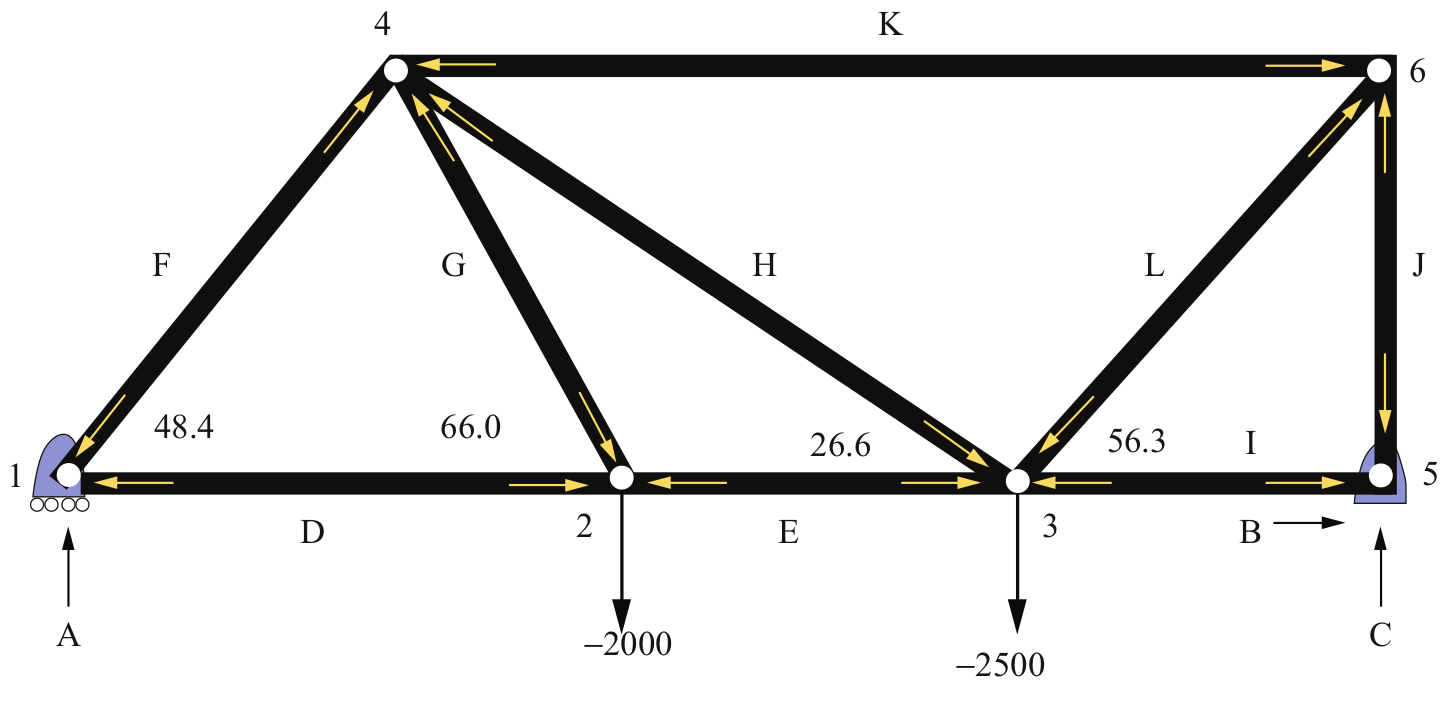
\includegraphics[width=0.7\linewidth]{fig_2_5}
	\caption{Truss problem.}
	\label{fig:fig_2_5}
\end{figure}

\begin{figure}
	\centering
	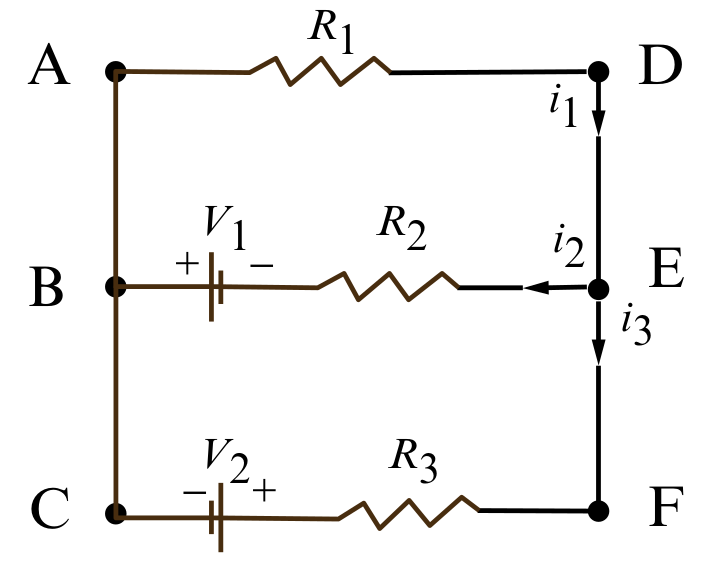
\includegraphics[width=0.5\linewidth]{fig_2_6}
	\caption{Circuit problem.}
	\label{fig:fig_2_6}
\end{figure}
\end{enumerate}

\end{document}